\chapter{Language Design}
\label{chap:LanguageDesign} 

AROS is designed to be descriptive and easy to use. Instead of making the programmer focus on the process of an agent and how it should achieve its goal, AROS allows the programmer to just describe what the environment and objectives are. Consequently, AROS computes the optimal process to achieve these objectives, since it is a detail that the programmer does not care about. Rather than writing a program that consists of a set of instructions (e.g. move left, go forward, etc.), the programmer writes a program that describes the environment (size of the area, position and size of obstacles) and the goal. AROS then finds the optimal path for the robot and creates a set of instructions it understands. 

\section{Grid layout}

A grid layout is the foundation of the map layout written in AROS. For a route to be computed, the programmer must have access to all relevant information about the space, which necessarily includes size and obstacles. Most likely, this information will already be presented as a grid. Therefore, recreating it into AROS is simply a matter of setting the dimensions and declaring the obstacles.
\par
A unit's dimension in the AROS grid space is necessarily arbitrary in order to allow different levels of resolution. To program a coffee delivery robot, the resolution of an obstacle might have to be 0.2 meters, for small objects and walls. For a drone or large spaces, however, it might be perfectly fine to keep the resolution at multiple meters per square, both to make programming easier and to reduce the complexity of the computation.
\par
The output of the program will be a series of "up", "down", "left" and "right" commands. These correspond to the robot's movements on the grid. So if the robot is at position (3,3) and receives a "down" command, it will go to the position (4,3). Receiving a "left" command afterwards moves it to (4,2). 
\par
We count on the software running on the robot having these aspects adjustable. Furthermore, an important assumption we make is that the robots are capable of perfectly executing their instructions. Via an array of sensors, if it receives the command "up", it will perform the operation. If it gets stuck or breaks down, it stops the execution. 

\section{Paradigm choice}

Programming languages can be classified based on their features into different paradigms, the main of which are \textit{imperative} and \textit{declarative}.
\par
The imperative programming paradigm allows the programmer to directly describe both the control flow and how the program is executed by changing the state of variables. This allows for constructs such as loops, which are risk-prone due to the fact that different parts of the program can change the same variable.
\par
Declarative programming focuses on the "what" and not the "how". The programmer specifies the properties of the result, not how to compute it. The decision to create a declarative programming language stems from the desire for the language to be a more straightforward and simple approach for declaring a map. Another reason is to differentiate it from the already existing and complex C-like code used for the Arduino platform.
\par
Logic and functional programming are subsets of declarative programming languages.
\par
Logic programming yields the results as the satisfying permutations of states in a defined universe of facts and rules. Using this paradigm would have our language consist of a series of facts describing the obstacles, and then a \textit{path} rule from start to end that would only be satisfied by a valid path.
\par
Functional programming returns the answer as the result of function applications. Due to the property of referential transparency, any function call can be any time replaced by its return value without affecting the result. This is important to our language since we want to always apply transformations going from one version to the map to the next while having the certainty that the previous version is unchanged.
\par
Functional programming also enables us to treat functions as first-class citizens and thus make our language more expressive.
\par
We have therefore decided on using a functional paradigm for AROS. The block structure of the code is familiar to people used to imperative programming, while actually being syntactic sugar for the purely functional "let..in" construct. Immutability enables the programmer to be certain that a defined shape will always stay the same shape, regardless of changes performed on it, without which debugging can possibly be extremely difficult.
\section{Informal overview}

\subsection{Basic types}

\subsubsection{Integer - \lstinline{int}}
    Integers are the basic (and only) numeric type in our language, which serves as the basic building block for higher compositional types.
    \newline \textbf{Examples:} \lstinline{0, 1, 2, 3, 100, 2000, -5, -123}
    
\subsubsection{Boolean - \lstinline{bool}}
    As with many programming languages, Boolean values that can either be true or false and can be used to define decisions and branching in the language.
    \newline \textbf{Examples:} \lstinline{true, false}

\subsubsection{Vector - \lstinline{vec}}
    Vectors in AROS are a composition of two integer components and represent a two-dimensional value, which can be used to define concepts such as size (as values of width and height) or a point on a grid (as coordinates on x and y-axes). 
    \newline \textbf{Examples:} \lstinline{<1,3>, <100,100>, <x,y>}

\subsubsection{List - \lstinline{[]}}
    Lists in AROS are a homogeneous collection of zero to many elements of an arbitrary type. In the context of AROS, they provide a basis for repetition and iteration using higher-order functions. Lists are defined recursively, with two components: a \textit{head} (first element) and a tail (a list containing the rest of the elements).
    \newline \textbf{Examples:}
    \begin{lstlisting}[language=aros,caption=List type examples]
        [int] ints = [1,2,3];
        [vec] vecs = [<1,2>, <3,4>, <5,6>];
    \end{lstlisting}

\subsubsection{Set - \lstinline{\{\}}}
    Similarly to lists, sets are also a collection of homogeneous elements, however, as with mathematical sets, they only allow distinct elements and do not maintain any particular order. Sets are very fundamental in AROS, as they provide the core structure for the definition of grid-based zone layouts. The need for sets as this core structure stems from the nature of defining zone layouts in the form of points on a grid, where non-distinct elements (overlapping points) would bear no meaning.
    \newline \textbf{Examples:} \lstinline|{<1,1>, <1,2>, <1,3>}, {1,2,3}, {true, false}|

\subsubsection{Function - \lstinline{[]}}
    Functions provide an abstraction over expressions, by encapsulating an arbitrary expression inside a local scope. This local scope contains the values of parameters, which are stated when a function is declared and passed into the local scope when the function is called, and the values of local variables declared inside the function body before the return expression. Both the function parameters and the local variables are optional.
    
\newblock
\par 
    In AROS, functions are treated as first-class citizens, and therefore can be used as parameters and/or return expressions of other functions.
    \newline \textbf{Example:}
    \begin{lstlisting}[language=aros,caption=Function type examples]
        (int -> int) addOne = (int) n -> int { n + 1 };
        int two = addOne(1); // two == 2
        
        (-> vec) makeConstVec = () -> vec {
            int x = 10;
            int y = 20;
            <x, y>
        };
        vec myVec = makeConstVec(); // myVec == <10,20>
        
        (int, int -> vec) makeDoublePoint = (int x, int y) -> vec {
           // local declarations 
           int doubled_x = x * 2;
           int doubled_y = y * 2;
           // expression
           <doubled_x, doubled_y>
        }; 
        vec point = makeDoublePoint(2, 2); // point == <4,4>
    \end{lstlisting}

\subsection{Operations}
\subsubsection{Basic arithmetic}
    AROS provides standard binary arithmetic operators for integers: \lstinline{+} for addition, \lstinline{-} for subtraction, \lstinline{*} for multiplication and \lstinline{/} for division. As integers are the only numeric type in AROS, division of two integers is defined as the nearest integer after their division: 
    \begin{equation*}
        \lfloor\frac{a}{b}\rceil
    \end{equation*}
    where $a$, $b$ are integers 
    \newline \textbf{Examples:}
    \begin{lstlisting}[language=aros, caption=Basic arithmetic examples]
        int one = 1;
        int two = one + one;   // two == 2 
        int four = two * two;  // four == 4 
        int four = two * two;  // four == 4 
        int three = 22 / 7;    // three == 3
    \end{lstlisting}
\subsubsection{Comparison operators}
    The comparison operators in AROS are also pretty standard compared to other mainstream programming languages. The equality operator $==$, which can be applied to all types, returns $true$ or $false$ if both operands are structurally equal. Similarly, there is also an inequality operator with symbol $!=$.
    \par The rest of the comparison operators only applied to integers and include:
    \begin{itemize}
        \item Greater than ($>$)
        \item Greater than or equal ($>=$)
        \item Less than ($<$)
        \item Less than or equal ($<=$)
    \end{itemize}
    \textbf{Examples:}
    
    \begin{lstlisting}[language=aros,caption=Comparison operator examples]
        // Integers
        5 == 5                           // true
        5 != 6                           // true
        2 > 1                            // true
        2 >= 1                           // true
        2 >= 2                           // true
        3 < 4                            // true
        3 <= 4                           // true
        3 <= 3                           // true
        
        // Booleans
        true == true                     // true
        true != false                    // true
        
        // Vectors
        <1,3> == <4,5>                   // false
        <1,3> != <4,5>                   // true
        <1,3> == <1,3>                   // true
        
        // Lists
        [1,2,3] == [1,2,3]               // true 
        [3,2,1] == [1,2,3]               // false
        [<1,2>, <3,4>] == [<1,2>, <3,4>] // true
        [<1,2>, <3,4>] == [<3,4>, <1,2>] // false
        
        // Sets
        {1,2,3} == {1,2,3}               // true 
        {3,2,1} == {1,2,3}               // true
        {<1,2>, <3,4>} == {<1,2>, <3,4>} // true
        {<1,2>, <3,4>} == {<3,4>, <1,2>} // true
        
    \end{lstlisting}
\subsubsection{Boolean logic}
    AROS also provides standard binary and unary operators for working with Boolean values, based on predicate logic. These are $and$ (true when both operands true), $or$ (true when either of operands true) and $not$ (negation). The $and$ and $or$ operators are short-circuited, therefore, the evaluation of the second operand may be skipped in case the result can be inferred from just the first operand.  
    \newline \textbf{Examples:}
    \begin{lstlisting}[language=aros,caption=Boolean logic examples]
        5 > 4 and 4 < 5       // true 
        5 > 4 or 5 < 4        // true
        not (5 > 4) and 5 > 4 // false
        not (5 > 4) or 5 > 4  // true
    \end{lstlisting}
\subsubsection{Vector operations}
    The integer arithmetic operators in AROS - $+$, $-$, $*$, $/$ - are overloaded to be also usable on vectors. Applying such operator on two vectors $v1$ and $v2$ will result in a new vector, whose components will be the results of applying the equivalent arithmetic operator pairwise to the respective components of $v1$ and $v2$. 
    \newline Apart from these operations, we can also access the $x$ and $y$ component of a vector by using the $vecx$ and $vecy$ keywords respectively, followed by the vector expression.
    \newline \textbf{Examples:}
    \begin{lstlisting}[language=aros,caption=Vector operation examples]
        vec v1 = <5,3>;
        vec v2 = <2,4>;
        vec added = v1 + v2;       // added == <7,7>
        vec subtracted = v1 - v2;  // subtracted == <3,-1>
        vec multiplied = v1 * v2;  // multiplied == <10,12>
        vec divided = v1 * v2;     // divided == <3,1>
        
        vec vector = <19,20>;
        int x = vecx vector;       // x == 19;
        int y = vecy vector;       // x == 20;
    \end{lstlisting}
\subsubsection{List operations}
    When it comes to (linked) lists in AROS, we can access the $head$ and $tail$ components of a list by using the special keywords `head` and `tail` respectively, followed by an expression of type list. To build a list dynamically, it is possible to use the cons operator ($:$) to prepend a new element onto a list. Additionally, we can also concatenate lists by using the append operator $++$. Given lists $l1$ and $l2$, the concatenation $l1 ++ l2$ evaluates to a new list, which begins with the elements of $l1$, which are followed by the elements of $l2$.
    \newline \textbf{Examples:}
    \begin{lstlisting}[language=aros,caption=List operation examples]
        [int] somePrimes = [13, 17, 19, 23, 29];
        int first = head somePrimes;      // first == 2
        [int] rest = tail somePrimes;       // rest == [3, 5, 7, 11]
        [int] morePrimes =  2 : 3 : 5 : 7 : 11 : []  // demonstrating the cons operator
        [int] myPrimes = morePrimes ++ somePrimes;
        // myPrimes == [2, 3, 5, 7, 11, 13, 17, 19, 23, 29]
    \end{lstlisting}

    
\subsubsection{Set operations}
    As mentioned before, sets are a fundamental feature of AROS and therefore the language natively provides several operators for sets.
    \par The most basic operators are union and intersection with their respective symbols $<>$ and $><$. These follow their mathematical definitions and can be applied to sets with elements of any type.
    \par \textbf{Examples:}
    \begin{lstlisting}[language=aros,caption=Union and intersection examples]
        // Integer sets
        {int} intSet1 = {1,2,3,4,5};
        {int} intSet2 = {4,5,6,7,8};
        {int} intUnion = intSet1 <> intSet2;
        // intUnion == {1,2,3,4,5,6,7,8}
        {int} intInters = intSet1 >< intSet2;
        // intInters == {4,5}
        
        // Vector sets
        {vec} vecSet1 = {<1,2>, <3,4>, <5,6>};
        {vec} vecSet2 = {<3,4>, <5,6>, <7,8>};
        {vec} vecUnion = vecSet1 <> vecSet2;
        // vecUnion == {<1,2>, <3,4>, <5,6>, <7,8>}
        {vec} vecInters = vecSet1 >< vecSet2;
        // vecInters == {<3,4>, <5,6>}
    \end{lstlisting}
    \par Moreover, there are two additional domain specific operators for sets of \textit{vectors}, to facilitate definitions and transformations in the context of points in a grid-based zone layout. Both of these take a set as their first argument, a vector as their second argument, and evaluate to a new set.
    \par The first one is the shift operator with symbol $>>$ which will evaluate to a set of vectors, equivalent to adding the vector argument of $>>$ to each vector in the set argument of $>>$. In the context of the zone, this will \textit{shift} or move the shape defined by the set of vectors.
    \par To give an example, we can show how we can build a shape out of 2 horizontal and 1 vertical lines, using the union and the shift operator: 
    \begin{lstlisting}[language=aros,caption=Examples of the shift operator, label=lst:shift-operator]
        {vec} vertical   = {<0,0>,<1,0>,<2,0>,<3,0>,<4,0>,<5,0>};
        {vec} horizontal = {<0,0>, <0,1>, <0,2>, <0,3>, <0,4>};
        
        // Make new (middle) vertical,
        // by shifting the original 2 coordinates to the right
        {vec} middleVertical = vertical >> (0, 2);
        // middleVertical == {<0,2>,<1,2>,<2,2>,<3,2>,<4,2>,<5,2>}
        
        // Make new (upper) horizontal,
        // by shifting the original 1 coordinate down
        {vec} upperHorizontal = horizontal >> (1, 0);
        // upperHorizontal == {<1,0>, <1,1>, <1,2>, <1,3>, <1,4>};
        
        // Make new (lower) horizontal,
        // by shifting the upper horizontal 3 coordinates down
        {vec} lowerHorizontal = upperHorizontal >> (3, 0);
        // lowerHorizontal == {<4,0>, <4,1>, <4,2>, <4,3>, <4,4>};
        
        // Group the lines into a single shape with union
        {vec} myShape = middleVertical 
                     <> upperHorizontal
                     <> lowerHorizontal;
        // myShape == {
        // <0,2>,<1,0>,<1,1>,<1,2>,<1,3>,<1,4>,<2,2>,
        // <3,2>,<4,0>,<4,1>,<4,2>,<4,3>,<4,4>,<5,2>
        //}
    \end{lstlisting}
    The set of vectors, $myShape$ built in this example, may be seen illustrated in the following figure:
    \begin{figure}[H]
        \centering
        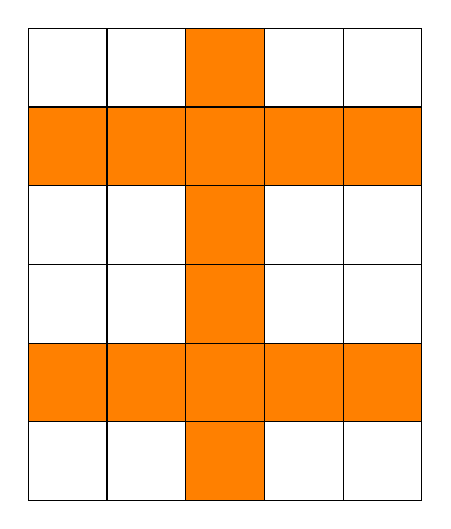
\begin{tikzpicture}[every node/.style={minimum size=1cm-\pgflinewidth, outer sep=0pt}]
            \draw[step=1cm, color=black] (0,0) grid (5,6);
            \node[fill=orange] at (2.5,5.5) {};
            
            \node[fill=orange] at (0.5,4.5) {};
            \node[fill=orange] at (1.5,4.5) {};
            \node[fill=orange] at (2.5,4.5) {};
            \node[fill=orange] at (3.5,4.5) {};
            \node[fill=orange] at (4.5,4.5) {};
            
            \node[fill=orange] at (2.5,3.5) {};
            \node[fill=orange] at (2.5,2.5) {};
            \node[fill=orange] at (2.5,1.5) {};
            \node[fill=orange] at (2.5,0.5) {};
            
            \node[fill=orange] at (0.5,1.5) {};
            \node[fill=orange] at (1.5,1.5) {};
            \node[fill=orange] at (3.5,1.5) {};
            \node[fill=orange] at (4.5,1.5) {};
        \end{tikzpicture}
        \caption{Illustration of shape represented by vector set $myShape$ built in \cref{lst:shift-operator}}
    \end{figure}
    \par The other operator specific to vector-sets is also contextual to defining shapes in the zone, called (and symbolized as) $crop$. The crop operator will remove any vectors from the set (first argument) based on their $x$ and $y$ components, if either of the following is true:
    \begin{itemize}
        \item $v_x > c_x - 1$
        \item $v_y > c_y - 1$
    \end{itemize}
    where $v_x$ , $v_y$ and $c_x$, $c_y$ are $x$ and $y$ components of a vector in the set and the vector argument of the $crop$ operation respectively.
    Effectively, this crops a shape (set of vectors) in a zone into a given width and height, specified in the $x$ and $y$ components of the vector argument of the operation. We can illustrate this on the previously created shape in the following code example:
    
    \begin{lstlisting}[language=aros,caption=Example of using the crop operator, label=lst:cropped-shape]
        {vec} myShapeCropped = myShape crop (5,3);
        // myShapeCropped == {
        // <0,2>,<1,0>,<1,1>,<1,2>,<2,2>,
        // <3,2>,<4,0>,<4,1>,<4,2>
        //}
    \end{lstlisting}
    
Which would result in the following shape:
    
    \begin{figure}[H]
        \centering
        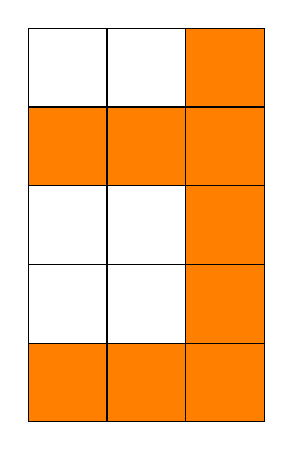
\begin{tikzpicture}[every node/.style={minimum size=1cm-\pgflinewidth, outer sep=0pt}]
            \draw[step=1cm, color=black] (0,0) grid (3,5);
            \node[fill=orange] at (0.5, 0.5) {};
            \node[fill=orange] at (1.5, 0.5) {};
            \node[fill=orange] at (2.5, 0.5) {};
            \node[fill=orange] at (2.5, 1.5) {};
            \node[fill=orange] at (2.5, 2.5) {};
            \node[fill=orange] at (2.5, 3.5) {};
            \node[fill=orange] at (2.5, 4.5) {};
            \node[fill=orange] at (0.5, 3.5) {};
            \node[fill=orange] at (1.5, 3.5) {};
        \end{tikzpicture}
        \caption{Illustration of shape represented by the cropped vector set $myShapeCropped$ built in \cref{lst:cropped-shape}}
    \end{figure}

\subsection{Constructs and Abstractions}
\subsubsection{Functions}
With AROS being a functional language, functions play a fundamental role as abstractions over expressions. Functions can be used to create an expression by constructing it gradually, in several steps (local declaration) in an isolated scope. Functions may be parameterized such that the resulting expression will be constructed and/or evaluated relative to the value(s) provided to the function.

\par{} The main primitive for defining and working with functions is a \textit{lambda} or anonymous function. Lambdas are treated equally to other expressions and act as literals of the function type, in the same way as there are literals for the vector or integer types. Consequently, a function \textit{definition} in AROS, is simply a variable declaration, with a function type and a value in the form of a lambda. An example of this may be seen in the following code listing:
    \begin{lstlisting}[language=aros, float=htb, caption= Function definition by binding a lambda literal to a name]
        (vec, vec -> [vec]) getSquareCoords = (vec bottomLeft, vec topRight) -> [vec] {
            vec topLeft = < (vecx bottomLeft), (vecy topRight) >;
            vec bottomRight = < (vecx topRight), (vecy bottomLeft) >;
            
            [bottomLeft, topLeft, topRight, bottomRight]
        };
    \end{lstlisting}
In the example, a function of type \lstinline{(vec, vec -> [vec])} (two vector parameters + vector list output), named \lstinline{getSquareCoords} has been defined. The function, given two vectors as coordinates of the bottom, left and top right corners of a square returns a list of all the four corners of that square. This example demonstrates how local scope and declarations can be used to define more complicated expression in a much more readable and writable way. 

\par{} Once a function is bound to a name (variable), it is possible to evaluate the function using function application and, for example, bind the evaluated value to a new variable:
    \begin{lstlisting}[language=aros, caption= Function application example]
        [vec] fiveByFive = getSquareCoords(<4,0>, <0,4>);
        // fiveByFive == [<4,0>, <0,0>, <0,4>, <4,4>]
    \end{lstlisting}
\par{} Alternatively, a lambda literal may be evaluated directly, without binding, such as in the following example:
    \begin{lstlisting}[language=aros,float=htb,caption= Direct application of a lambda literal]
        int twoSquared = ((int n) -> int { n * 2 })(2);
        // twoSquared == 4
    \end{lstlisting}

\subsubsection{Conditional expressions}
Decisions based on boolean expressions are facilitated using two main constructs: \lstinline{if} expressions and \lstinline{cond} expressions. As the naming suggests, as the majority of AROS, these are also expressions and therefore may be directly evaluated and bound to variables.

\par As is standard in many programming languages, \lstinline{if} expressions consists of three components: the \textit{condition} and two expressions of same type, call them \lstinline{e1} and \lstinline{e1}. When the entire if expression is evaluated, it will result in either \lstinline{e1} or \lstinline{e2}, based on whether the condition evaluated to \lstinline{true} or \lstinline{false} respectively. An example may be seen in the listing below: 
    \begin{lstlisting}[language=aros, caption= Example of an if expression]
        int x = 10;
        vec a = if (x < 10) { 
            <0,0>    
        } else {
            <10, 10>
        };
        // a == <0,0>
    \end{lstlisting}

\par AROS also makes available another conditional expression, \lstinline{cond}, for situations where the branching consists of more than two branches (and therefore more than one conditions). While this is technically possible to do by nesting \lstinline{if} expressions, \lstinline{cond} provides this functionality in a more concise syntax, giving the users more readability and writability. The following listing contains an example of this construct:

    \begin{lstlisting}[language=aros, caption= Example of a cond expression]
        int x = 100;
        vec a = cond {
            ((x > 0) and (x < 10)) {
                <0,0>
            }
            ((x >= 10)  and (x < 20)) {
                <10,10>
            }
            ((x >= 20) and (x < 30)) {
                <20,20>
            }
            otherwise { <100,100> }
        }; // a == <100, 100>
    \end{lstlisting}
    
\subsubsection{Recursion and Iteration}
In order to execute repetitive computations in a functional style, recursion (function calling itself) can be used. For example, the following code listing includes an implementation of calculating the n-th Fibonacci number recursively:
    \begin{lstlisting}[language=aros, label=lst:fibr, caption= Recursive implementation of calculating n-th Fibonacci number]
        (int -> int) fibr = (int n) -> int {
            cond {
               ((n == 0) or (n == 1)) { n } 
               otherwise { 
                    fibr(n-1) + fibr(n-2)
               }
            }
        }
        int fib5 = fibr(5);
        // fib10 == 55
    \end{lstlisting}

\par{} While \cref{lst:fibr} is sufficient to illustrate recursion, it is a very inefficient implementation. The complexity of this implementation is exponential, due to the repeated recursions stemming from line 5 in \cref{lst:fibr}. The complexity of calculating n-th Fibonacci number can be significantly increased by using an iterative approach. Even though AROS is a functional language and therefore does not support iterative control structures such as a $while$ loop or a $for$ loop, we can make an iterative implementation by passing accumulator values in recursion. The example in 

\newblock

    \begin{lstlisting}[language=aros, label={lst:fibi}, caption= Iterative implementation of calculating n-th Fibonacci number]
        (int, int, int -> int) fibi_h = (int n, int a, int b) -> int {
            cond {
               (n == 0) { a } 
               (n == 1) { b }
               otherwise { 
                    fibi_h(n-1, b, a + b)
               }
            }
        };
        
        (int -> int) fibi = (int n) -> int {
            fibi_h(n, 0, 1)
        };
        
        int fib5 = fibi(5);
        // fib10 == 55
    \end{lstlisting}

\subsubsection{Generic higher-order functions}

\par 
In a functional language paradigm, higher-order function, such as map, filter and fold, are commonly used to solve particular problems. They are in fact, so frequent and versatile, that we have decided to incorporate them into the syntax of AROS. 

\par 
Map takes a function $f$ and a list $l_1$ and applies that function $f$ to every element in the list $l_1$, producing a new list $l_2$. The type scheme of a map is $((\alpha \rightarrow \beta), [\alpha] \rightarrow [\beta])$, meaning that the argument of function $f$ must have the same type as element of list $l_1$ and the return type of function $f$ must be the same as the type of the element of $l_2$. The following example utilizes map to shift every x coordinate of a vector in a list by 1.

\newblock 
\begin{lstlisting}
    (vec -> vec) f = (vec v) -> vec {
        int x = vecx v;
        int y = vecy v;
        <x + 1, y>
    };
    
    [vec] l = [<1,1>, <1,2>, <1,3>];
    
    [vec] new_l = map(f, l); 
    //new_l == [<2,1>, <2,2>, <2,3>]
\end{lstlisting}

\newblock
\par 
Filter takes a predicate (a function $f$, which returns a boolean value) and a list $l_1$ and returns a list $l_2$, consisting of elements of $l_1$ that satisfy the predicate. The type scheme of a filter is $((\alpha \rightarrow Bool), [\alpha] \rightarrow [\alpha])$, meaning that the type of argument of $f$ and the type of elements of both lists $l_1$ and $l_2$ must be equal. The following example utilizes filter to filter out empty sets from a list.

\newblock 
\begin{lstlisting}
    ({vec} -> bool) f = ({vec} s) -> bool {
        s != {}
    };
    
    [{vec}] l = [{<1,1>, <1,2>, <1,3>}, {}, {<0,0>}, {}];
    
    [vec] new_l = filter(f, l); 
    //new_l == [{<1,1>, <1,2>, <1,3>}, {<0,0>}]
\end{lstlisting}

\newblock
\par
A fold (right) takes a function, a starting value (an accumulator) and a list to fold up. The function itself takes two parameters. The function is called with the accumulator and the last element and produces a new accumulator. Then, the function is called again with the new accumulator and the now new last element, and so on. Once we have walked over the whole list, only the accumulator remains, which is what we have reduced the list to. \cite[p. 61]{learn-you-a-haskell-for-great-good} The type scheme of fold right is $((\alpha, \beta \rightarrow \beta), \beta, [\alpha] \rightarrow \beta)$. The following example is an implementation of the above map, using the right fold.

\begin{lstlisting}
    ((vec -> vec), [vec] -> [vec]) map' = ((vec -> vec) f, [vec] l) -> [vec]{
        (vec, [vec] -> [vec]) f' = (vec h, [vec] a) -> [vec] {
            f(h) : a
        }
        foldr(f', [], l)
    }
\end{lstlisting}

\subsubsection{Domain specific constructs}
As mentioned in the previous sections, the key objective of every program written in AROS is to define the map, obstacles and route from the robot's current position to its goal. Therefore, there are two specific constructs that have to be present at the end of every program written in AROS - the grid and route definitions. 

 \par
 The grid definition begins with a $\textit{grid}$ keyword followed by two expressions separated by a comma. The first expression represents the size of the grid and therefore must evaluate to a vector. The second expression must evaluate to a set of vectors because it represents all the obstacles on the grid. Any obstacles defined beyond the size of the grid will simply be discarded. 
 
 \par 
 The route definition begins with a $\textit{route}$ keyword, which is similarly followed by two expressions, separated by a comma. The expressions define the starting and ending position of the path that a robot has to undertake. Both of these expressions have to evaluate to a vector. The following demonstrates the usage of these constructs.
 
 \newblock
 
\begin{lstlisting}
    vec size = <5,5>;
    {vec} obstacles = {<1,1>,<2,2>,<3,3>};
    vec start = <0,0>;
    vec end = <4,4>
    
    grid size, obstacles
    route start, end
\end{lstlisting}
\section{Formal specification}\label{section:Specification}

\subsection{Abstract grammar}
\label{sec:abstract-grammar}

\par
In this section, we give a formal description of the AROS language, such that it is clear which programs are syntactically valid and which are not. We first define it by means of the abstract grammar. 

\par
Abstract grammar is a context-free grammar, which provides a clearer, simplified syntactic description of the language. However, compared to a concrete grammar, it may be ambiguous and it is not concerned with e.g. operator precedence, etc. The abstract syntax is defined by a collection of syntactic categories and a finite set of formation rules for every syntactic category.

\par
The abstract grammar of AROS consists of the following syntactic categories:


\begin{align*}
    & i \in \mathbf {Int} - \text{Integers} \\
    & b \in \mathbf {Bool} - \text{Booleans} \\
    & x \in \mathbf {Var} - \text{Variables} \\ 
    & e \in \mathbf {Exp} - \text{Expression} \\
    & T \in \mathbf {Type} - \text{Types} \\
    & P \in \mathbf {Params} - \text{Function parameters} \\
    & L \in \mathbf {Lambda} - \text{Lambda expression} \\
    & B \in \mathbf {Block} \\
    & FA \in \mathbf {FunctionApplication} \\
    & D \in \mathbf {Dec} - \text{Declaration} \\
    & G \in \mathbf {GridDef} - \text{Grid definition} \\
    & R \in \mathbf {RouteDef} - \text{Route definition} \\
    & Prog \in \mathbf {Program}
    &&&
\end{align*}

\newblock
\par
An arbitrary element of a syntactic category is represented by meta-variables. For example, $e$ is a meta-variable for expression, L is a meta-variable for lambda, etc. Members of the above mentioned syntactic categories are defined by sets of formation rules:

\begin{flalign*}
    & T ::= int\\
        &\quad \quad \: | \: bool \\
        &\quad \quad \: | \: vec \\
        &\quad \quad \: | \: [T] \\
        &\quad \quad \: | \: \{T\} \\
        &\quad \quad \: | \: ( [T,]^* T \rightarrow T ) \\
        &\quad \quad \: | \: ( \rightarrow T ) \\ \\
    & e ::= x \\
        & \quad \quad | \: i \\
        & \quad \quad | \: b \\
        & \quad \quad | \: <e,e> \\
        & \quad \quad | \: [ [e,]^* e]\\
        & \quad \quad | \: [ \: ] \\
        & \quad \quad | \: \{ [e,]^* e \} \\
        & \quad \quad | \: \{ \: \} \\
        & \quad \quad | \: (e) \\
        & \quad \quad | \: o_1 \: e \\
        & \quad \quad | \: e \: o_2 \: e \\
        & \quad \quad | \: L \\
        & \quad \quad | \: FA \\
        & \quad \quad | \: if(e) \: B \: else \: B\\
        & \quad \quad | \: cond\{\: [(e) \: B]^+ \: otherwise \: B \} \\
        & \text{where } \\
        & \quad o_1 \in \{ not, \: head, \: tail, \: vecx, \: vecy\} \\
        & \quad o_2 \in \{ +, \: -, \: *, \: / , \: ++, \: : , \: <> , \: >< , \: >> , \: crop , \: and, \: or , \: > , \: < , \: >= , \: <= , \: == , \: != \} \\ \\
    & FA ::= x \: P \\
         & \: \: \: \: \quad \quad | \: L \: P \\
         & \: \: \: \: \quad \quad | \: map (e, e) \\
         & \: \: \: \: \quad \quad | \: filter (e, e) \\
         & \: \: \: \: \quad \quad | \: fold (e, e, e)
    &&&
\end{flalign*}

\begin{flalign*}
    & P ::= ([e,]^* \: e) \: | \: ( \lambda ) \\
    & B ::= \{ \: D \: e \} \\ \\
    & L ::= ([T \: x,]^* \: T \: x) \rightarrow T \: B \\
        & \quad \quad | \: \: (\lambda) \rightarrow T \: B \\ \\
    & D ::= T \: x = e; \: D \: | \: \lambda \\
    & G ::= grid \: e, \: e \\
    & R ::= route \: e, \: e \\
    & Prog ::= D \: G \: R\\
    &&&
\end{flalign*}

\par 
The function type $([T,]^* \: T) \rightarrow T$, is just syntactic sugar, allowing multiple input parameters. However, every function type can be redefined by its equivalent curried form. Therefore the type $(T_1, T_2, T_3 \rightarrow \: T_4)$, can be defined as $(T_1 \rightarrow \: (T_2 \rightarrow \: (T_3 \rightarrow \: T_4)))$. This can be illustrated on the following two functions $f$ and $f'$.

\newblock
\begin{lstlisting}[language=aros]
    (int, int, int -> int) f = 
        (int x, int y, int z) -> int {
            x * y * z
    }
    
    (int -> (int -> (int -> int))) f' =
        (int x) -> int {
           (int y) -> int {
                (int z) -> int {
                    x * y * z
                }
            }
        }
\end{lstlisting}

\newblock
\par
We assume that elements of $\textbf{Int}$ are integers, elements of $\textbf{Bool}$ are either $true$ or $false$ and an element of $\textbf{Var}$ is any string containing only letters of Latin alphabet, Arabic numerals and symbol $\_$, starting with a lowercase letter. We can define these categories by means of regular expressions:


\begin{align*}
    & b :== true \: | \: false \\
    & i :== [-]?[1-9][0-9]^* \: | \: 0 \\
    & x :== [a-z][a-zA-Z0-9\_]^* \\
    &&&
\end{align*}

\subsection{Type system}
\label{sec:design:formal:type-system}
\par
As informally described in section XY, values of expressions in the language can be of type integer, boolean, vector, set, list or a function. Types are defined formally using the formation rules in table XYY. Such recursive definition of lists and sets allows nesting, so that a ``list of sets of integers'', $[ \{int\} ]$, is a valid type. 

\par 
Similarly, the same principle applies to functions. They can accept other functions as parameters as well as return functions. While a function is only allowed to return one expression of a given type, it can accept an arbitrary number of input parameters, or no parameters at all. The following are examples of function types allowed in AROS:


\begin{align*}
    & (int \rightarrow bool)\\
    & (int, int \rightarrow vec)\\
    & ((int \rightarrow bool), [int] \rightarrow [bool])\\
    & ( \rightarrow (\{vec\} \rightarrow [vec]))\\
    &&&
\end{align*}

\par
Therefore, the set of valid types in AROS $\textbf{Type}$, is infinite: 

\begin{align*}
    Type = \{ int, bool, vec, [int], [bool], [vec], [[int]], \cdots, (int \rightarrow int), \cdots, (int,(int \rightarrow bool) \rightarrow bool), \cdots \}
\end{align*}

\newblock
\par
Furthermore, we can define two subsets of $\textbf{Type}$:

\begin{align*}
    & \mathbf{SType} \subset \mathbf{Type} - \text{Standard type} \\
    & \mathbf{FType} \subset \mathbf{Type} - \text{Function types} \\  
    & where \: \mathbf{FType} \cap \mathbf{SType} = \emptyset \\
    &&&
\end{align*}

Formation rules for each subset can be defined as follows:

\begin{align*}
    & T_s ::= int \: | \: bool \: | \: vec \: | \: [T] \: | \: \{T\} \text{,where } T_s \in \mathbf{SType} \\
    & T_f ::= ([T,]^*T \rightarrow T) \: | \: (\rightarrow T) \text{,where } T_f \in \mathbf {FType} \\
    &&&
\end{align*}

\newblock
\par
According to the abstract grammar, it is syntactically correct to write an expression such as $10+\{true, false\} $. Such expression, of course, does not make sense and it is hard to imagine how a number 10 can be added to a set of Boolean values. The goal of a type system is to ensure type safety by disallowing such expressions.

\par
Declarations of variables is an essential language construct in AROS. It is necessary to keep track of types of these variables so that we will be able to correctly evaluate expressions containing them. To do this, we use \textit{E} as the type environment. The type environment $E$ can be defined as a partial function: 

\begin{align*}
    E: Var \rightharpoonup Type
\end{align*}

where
\begin{itemize}
    \item $Var$ is a set of declared variables
    \item $Type$ is a set of types
    \newline
\end{itemize}

\par
To update a type environment with a new declaration of variable $x$ of type $T$ we write $E[x \longmapsto T]$, obtaining an updated environment $E'$ defined by: 

\begin{align*}
    E'(y) = \begin{cases} E(y) &\mbox{if } y \neq x \\ 
   T &\mbox{if } y = x \end{cases}
\end{align*}

We can now define type rules that describes how types are assigned to syntactic entities. We employ type judgements of the form:     

\begin{align*}
    E \vdash e : T
\end{align*}

where:
\begin{itemize}
    \item $E$ is a type environment - mapping from declared variables to their types
    \item $e$ is an expression
    \item $T$ is a type
\end{itemize}

\par
In other words, the above definition states that the expression $e$ has type $T$ relative to the type environment $E$.\newline

\par
Type judgements are combined into type rules of the following form:

\begin{align*}
    {\dfrac{J_1; J_2;...;J_n}{J}}
\end{align*}

where:
\begin{itemize}
    \item $J_i$ for $1 \leq i \leq n$ is a premise of the type rule
    \item $J$ is a conclusion of the type rule
\end{itemize}

\par
So that if all the type judgements $J_i$ hold, the conclusion J also holds. We can now describe our type system as follows: 
\begin{flalign}
    & [VAR_{EXP}]\quad {\dfrac{E(x) = T}{E \vdash x \colon T}} &
\end{flalign}

\begin{flalign}
    & [PAR_{EXP}]\quad {\dfrac{E \vdash x \colon T}{E \vdash(x) \colon T}} &
\end{flalign}

\begin{flalign}
    & [INT_{EXP}]\quad {E \vdash i \colon int} &
\end{flalign}

\begin{flalign}
    & [INT\_OP_{EXP}]\quad {\dfrac{E \vdash e_1 \colon int; E \vdash e_2 \colon int}{E \vdash e_1 \:  o \:  e_2 \colon int}}\text{, where } o \in \{+,-,*,/\} &
\end{flalign}

\begin{flalign}
    & [BOOL_{EXP}]\quad {E \vdash b \colon bool} &
\end{flalign}

\begin{flalign}
    & [BOOL\_OP_{EXP}]\quad {\dfrac{E \vdash e_1 \colon bool;E \vdash e_2 \colon bool}{E \vdash e_1 \: o \: e_2 \colon bool}}\text{, where } o \in \{and, or\} &
\end{flalign}

\begin{flalign}
    & [BOOL\_COMP_{EXP}]\quad {\dfrac{E \vdash e_1 \colon int;E \vdash e_2 \colon int}{E \vdash e_1 \: o \: e_2 \colon bool}}\text{, where } o \in \{>,<,>=,<=,==,!=\} &
\end{flalign}

\begin{flalign}
    & [BOOL\_NEGATION_{EXP}]\quad {\dfrac{E \vdash e \colon bool}{E \vdash not \: e \colon bool}} &
\end{flalign}

\begin{flalign}
    & [VEC_{EXP}]\quad {\dfrac{E \vdash e_1 \colon int;E \vdash e_2 \colon int}{E \vdash \langle e_1,e_2 \rangle  \colon vec }} &
\end{flalign}

\begin{flalign}
    & [VEC\_UOP_{EXP}]\quad {\dfrac{E \vdash e \colon vec}{E \vdash o \: e \colon int}}\text{, where }o \in \{vecx, vecy \} &
\end{flalign}

\begin{flalign}
    & [VEC\_BOP_{EXP}]\quad {\dfrac{E \vdash e_1 \colon vec; E \vdash e_2 \colon vec}{E \vdash e_1 \: o \: e_2 \colon vec}}\text{, where }o \in \{+,-,*,/ \} &
\end{flalign}

\begin{flalign}
    & [VEC\_SCAL_{EXP}]\quad {\dfrac{E \vdash e_1 \colon int;E \vdash e_2 \colon vec}{E \vdash e_1 \: * \: e_2 \colon vec}} &
\end{flalign}
\label{page:empty-set-list}
\begin{flalign}
    & [EMPTY\_LIST_{EXP}]\quad E \vdash [\text{ }] : [T] &
\end{flalign}

\begin{flalign}
    & [LIST\_CONS_{EXP}]\quad {\dfrac{E \vdash e_1 \colon T; E \vdash e_2 \colon [T]}{E \vdash e_1 \: \colon \: e_2 \colon [T]}} &
\end{flalign}

\begin{flalign}
    & [LIST\_APPEND_{EXP}]\quad {\dfrac{E \vdash e_1 \colon [T];E \vdash e_2 \colon [T]}{E \vdash e_1  ++  e_2 \colon [T]}} &
\end{flalign}

\begin{flalign}
    & [LIST\_HEAD_{EXP}]\quad {\dfrac{E \vdash e \colon [T]}{E \vdash head \text{ } e \colon T}} &
\end{flalign}

\begin{flalign}
    & [LIST\_TAIL_{EXP}]\quad {\dfrac{E \vdash e \colon [T]}{E \vdash tail \text{ } e \colon [T]}} &
\end{flalign}

\begin{flalign}
    & [SET_{EXP}]\quad {\dfrac{E \vdash e \colon T}{E \vdash \{e\} \colon \{T\}}} &
\end{flalign}

\begin{flalign}
    & [EMPTY\_SET_{EXP}]\quad {E \vdash \{ \text{ }\} \colon \{T\}} &
\end{flalign}

\begin{flalign}
    & [SET\_OP_{EXP}]\quad {\dfrac{E \vdash e_1 \colon \{T\}; E \vdash e_2 \colon \{T\}}{E \vdash e_1 \: o \: e_2 \colon \{T\}}}\text{, where }o \in \{\cup, \cap\} &
\end{flalign}

\begin{flalign}
    & [VECTOR\_SET\_OP_{EXP}]\quad {\dfrac{E \vdash e_1 \colon \{vec\}; E \vdash e_2 \colon vec}{E \vdash e_1 \: o \: e_2 \colon \{vec\}}}\text{, where }o \in \{\gg, *,crop\} &
\end{flalign}

\begin{flalign}
    & [LAMBDA^1_{EXP}]\quad {
    \dfrac
    {E[x_1 \longmapsto T_1, \cdots, x_n \longmapsto T_n] \vdash B \colon T_r}
    {E \vdash (T_1 \: x_1, \cdots,\: T_n \: x_n) \rightarrow \: T_r \: B \colon ( T_1, \cdots, T_n \rightarrow T_r ) }} &
\end{flalign}

\begin{flalign}
    & [LAMBDA^2_{EXP}]\quad {
    \dfrac
    {E \vdash B \colon T}
    {E \vdash ( \lambda) \rightarrow T \: B \colon T }} &
\end{flalign}

\begin{flalign}
    & [IF_{EXP}]\quad {\dfrac{E \vdash e \colon bool; E \vdash B_1 \colon T; E \vdash B_2 \colon T}{E \vdash if(e) B_1  \text{ else } B_2 \colon T}} &
\end{flalign}

\begin{flalign}
    & [COND_{EXP}]\quad {\dfrac{E \vdash e_1 \colon bool; \cdots ; E \vdash e_n \colon bool ; E \vdash B_1 \colon T; \cdots ; E \vdash B_n \colon T, E \vdash B_o \colon T}{E \vdash cond\{ (e_1) B_1 \cdots (e_n) B_n \text{ otherwise } B_o\} \colon T}} &
\end{flalign}

\begin{flalign}
    & [APP\_VAR_{EXP}]\quad {\dfrac
        {E \vdash x \colon (T_1, \cdots,T_n \rightarrow T_r); E \vdash P \colon T_1, \cdots, T_n}
        {E \vdash x \: P \colon T_r}
    } &
\end{flalign}

\begin{flalign}
    & [APP\_LAMBDA_{EXP}]\quad {\dfrac
        {E \vdash L \colon (T_1, \cdots,T_n \rightarrow T_r); E \vdash P \colon T_1, \cdots, T_n}
        {E \vdash L \: P \colon T_r}
    } &
\end{flalign}

\begin{flalign}
    & [APP\_EMPTY_{EXP}]\quad {\dfrac
        {E \vdash L \colon (\rightarrow T)}
        {E \vdash L \: (\lambda) \colon T}
    } &
\end{flalign}

\begin{flalign}
    & [APP\_MAP_{EXP}]\quad {\dfrac
        {E \vdash e_1 \colon (T_1 \rightarrow T_2); E \vdash e_2 \colon [T_1]}
        {E \vdash map(e_1, \: e_2) \colon [T_2]}
    } &
\end{flalign}

\begin{flalign}
    & [APP\_FILTER_{EXP}]\quad {\dfrac
        {E \vdash e_1 \colon (T \rightarrow Bool); E \vdash e_2 \colon [T]}
        {E \vdash filter(e_1, \: e_2) \colon [T]}
    } &
\end{flalign}

\begin{flalign}
    & [APP\_FOLD_{EXP}]\quad {\dfrac
        {E \vdash e_1 \colon (T_1, \: T_2 \rightarrow T_1); E \vdash e_2 \colon T_1; E \vdash e_3 \colon [T_2]}
        {E \vdash fold(e_1, \: e_2, \: e_3) \colon T_1}
    } &
\end{flalign}

\begin{flalign}
    & [PARAMS]\quad {\dfrac
        {E \vdash e_1 \colon T_1; \cdots; E\vdash e_n \colon T_n}
        {E \vdash (e_1,\cdots,e_n) \colon T_1,\cdots,T_n}
    }
    &
\end{flalign}

\begin{flalign}
    & [BLOCK]\quad {\dfrac
        {E \vdash D \: e \colon T}
        {E \vdash \{ D \: e \} \colon T}
    } &
\end{flalign}

\begin{flalign}
    & [EMPTY_{DEC}]\quad {
        \dfrac
        {E \vdash G \colon ok; E \vdash R \colon ok}
        {E \vdash \lambda \: G \: R \colon ok}
    } &&&
\end{flalign}

\begin{flalign}
    & [VAR_{DEC}]\quad { 
        \dfrac
        {E[x \longmapsto T] \vdash D \: G \: R \colon ok; E \vdash e \colon T}
        {E \vdash T \: x =e; \: D \: G \:R \colon ok}
        \text{,where } T \in \mathbf{SType}
    } &&&
\end{flalign}

\begin{flalign}
    & [VAR\_REC_{DEC}]\quad 
    {
        \dfrac
        {E[x \longmapsto T] \vdash D \: G \: R \colon ok; E[x \longmapsto T] \vdash e \colon T}
        {E \vdash T \: x =e; \: D \:G \:R \colon ok}
        \text{,where } T \in \mathbf{FType}
    }&&&
\end{flalign}

\begin{flalign}
    & [EMPTY\_BLOCK_{DEC}]\quad {
        \dfrac
        {E \vdash e \colon T}
        {E \vdash \lambda \: e \colon T}
    }&&&
\end{flalign}

\begin{flalign}
    & [VAR\_BLOCK_{DEC}]\quad {
        \dfrac
        {E[x \longmapsto T] \vdash D \: e' \colon T';E\vdash e \colon T}
        {E \vdash T \: x = e; D \: e' \colon T'}
        \text{,where } T \in \mathbf{SType}
    }&&&
\end{flalign}

\begin{flalign}
    & [VAR\_BLOCK\_REC_{DEC}]\quad
    {
        \dfrac
        {E[x \longmapsto T] \vdash D \: e' \colon T';E[x \longmapsto T]\vdash e \colon T}
        {E \vdash T \: x = e; D \: e' \colon T'}
        \text{,where } T \in \mathbf{FType}
    }&&&
\end{flalign}

\begin{flalign}
    & [GRID]\quad {\dfrac
        {E \vdash e_1 \colon vec; E \vdash e_2 \colon \{vec\}}
        {E \vdash grid \: e_1, \: e_2 \colon ok}
    } &
\end{flalign}

\begin{flalign}
    & [Route]\quad {\dfrac
        {E \vdash e_1 \colon vec; E \vdash e_2 \colon vec}
        {E \vdash route \: e_1, \: e_2 \colon ok}
    } &
\end{flalign}

\newblock
\par
After defining our type system, we can easily observe that the previously mentioned expression: $10 + \{true, false\}$, is a bad expression that is not typable because there is no type rule defining how to add an integer to a set of Booleans.

\par
Some type rules are applicable to any types. For example, the type rule 2.23 states, that a $if expression$ can be of any type, as long as its condition $b$ has type Boolean and both blocks are of the same type. 

\par
We can now employ these type rules and claim that the function on SNIPPET-XY has type $(vec, int \rightarrow [vec])$ and its declaration is $ok$. 

\newblock
\begin{lstlisting}[language=aros]
(vec, int -> [vec]) hr = 
    (vec s, int l) -> [vec] {
        if(l == 0){
            []
        }
        else{
            int l'= l-1;
            int x = vecx s;
            int y = vecy s + l';
            <x, y> : hr(s, l')
        }
}
\end{lstlisting}

\newblock
\par
However, for simplicity reasons, the sample program contains neither a grid nor a route definition and only consists of a single declaration. To validate it, we have to alter global declaration rules, such that, they do not require a grid and route after declarations:

\begin{flalign}
    & [VAR\_TEMP\_REC_{DEC}]\quad 
    {
        \dfrac
        {E[x \longmapsto T] \vdash \text{D} \colon ok; E[x \longmapsto T] \vdash e \colon T}
        {E \vdash T \: x =e; \: D \colon ok}
        \text{,where } T \in \mathbf{FType}
    }&&&
\end{flalign}

\begin{flalign}
    & [EMPTY\_TEMP_{DEC}]\quad {E \vdash \lambda \colon \text{ok}} &&&
\end{flalign}

\begin{align*}
        \dfrac
        {
            \dfrac
            {
            }
            {E[hr \longmapsto (vec, int \rightarrow [vec])] = E^1 \vdash \lambda \colon ok;}
            \quad
            \dfrac
            {
                \dfrac
                {...}
                {E^1[s \longmapsto vec, l \longmapsto int] = E^2 \vdash Block_1 \colon [vec]}
            }
            {E^1 \vdash (vec \: s,\: int \:l) \rightarrow [vec] \:  Block_1 \colon (vec, int \rightarrow [vec])}
        }
        {
            E \vdash (vec, int \rightarrow [vec]) hr = (vec \: s,int \: l) \rightarrow [vec] \: Block_1 \colon ok 
        }
\end{align*}

where $Block_1$ is a substitution for the body of the function $hr$.

\newblock
\par
In order to employ the appropriate type rule, we have to examine the nature of this declaration. It is easy to observe that $hr$ is a function. However, it is also a recursive function, because it is applied directly in its body. To deal with this, we have to use a type rule restricted to the functional declaration - $[VAR\_TEMP\_REC_{DEC}]$. The difference between $[VAR\_REC_{DEC}]$ (or the altered $[VAR\_TEMP\_REC_{DEC}]$) and $[VAR_{DEC}]$ is that the former updates the type environment for both premises. Therefore, when the derivation tree reaches the function application, the variable $hr$ can be looked up in the type environment. Such recursive declarations have been restricted to functional types, since declarations such as $int \text{ } x = 5 * x$ do not make sense in a context of declarative programming language, without assignments or mutations. 

\par
$E^1$ is the updated environment $E$ with variable $hr$ of type $(vec,int \rightarrow [vec])$. Since there are no other declarations, we can apply the $[EMPTY\_TEMP_{DEC}]$ rule, reaching an axiom stating that an empty declaration is $ok$. Furthermore, we have to verify that the expression on the right-hand side of the declaration does have the stated type. Employing the $[LAMBDA^1_{EXP}]$ rule, we first update the environment $E^1$ with function parameters and their types. It is important to note, that if there were other declarations in the sample program, this update would not leak to other branches of the derivations tree, preserving the scope of the function. Next, we have to verify that the function body evaluates to the expected return type. To progress the right branch of the derivation tree, we substitute back the function body for $Block_1$.



\begin{align*}
    \dfrac
    {
        \dfrac
        { \dfrac
        {
            \dfrac{\dfrac{}{E^2(l) = int}}{E^2 \vdash l \colon int;}
            \dfrac{}{E^2 \vdash 0 \colon int}
        }
        {E^2 \vdash l == 0 \colon bool;}
        \quad
        \dfrac
        {\:}
        {E^2 \vdash [ \: ] \colon [vec];} 
        \quad
        \dfrac
        {...}
        {E^2 \vdash Block_2 \colon [vec]}}
        {E^2 \vdash if (l == 0) \{ [ \: ] \} \: else \: Block_2 \colon [vec]}
    }
    {
        E^2 \vdash \{ \: if (l == 0) \{ [ \: ] \} \: else \: Block_2 \: \} \colon [vec]
    }
\end{align*}

where $Block_2$ is a substitution for the body of the else block.

\par
To continue the derivation we first use the $[BLOCK]$ rule to remove the outer curly brackets. Then, by application of the $[IF_{EXP}]$ type rule, we check that the condition is of type Bool and that both blocks return type $[vec]$. To validate the type of the Boolean expression, we employ the $[BOOL\_COMP_{EXP}]$ rule and check that both variable $l$ and $0$ are integers. The variable $l$ can be looked up in the type environment $E^2$ since:

\begin{flalign}
    E^2 = hr:(vec,int \rightarrow [vec]), s:vec, l:int   
\end{flalign}

\newblock
\par
The first block of the $if expression$ is an axiom $[EMPTY\_LIST_{EXP}]$. We can now substitute back $Block_2$ and continue the derivation.

\begin{align*}
    \dfrac
    {
        \dfrac
        {
        \dfrac
            {\dfrac{\dfrac{}{E^2(l) = int}}{E^2 \vdash l \colon int;}
             \dfrac{}{E^2 \vdash 1 \colon int}
            }
            {E^2 \vdash l - 1 \colon int;}
        \dfrac
            {
                \dfrac
                {
                    \dfrac
                    {
                        \dfrac
                        {}
                        {E^3(s) = vec}
                    }
                    {E^3 \vdash s \colon vec}
                }
                {E^3 \vdash vecx \: s \colon int; }
                \quad
                \dfrac
                {...}
                {E^3[x \longmapsto int] = E^4 \vdash Decs_1 \: Exp_1 \colon [vec]}
            }
            {E^2[l' \longmapsto int] = E^3 \vdash int \text{ } x = vecx  \text{ }  s; Decs_1 \: Exp_1 \colon [vec]}
        }
        {E^2 \vdash int \: l' = l - 1; int \text{ } x = vecx \: s; Decs_1 Exp_1 \colon [vec]}
    }
    {E^2 \vdash \{ \: int \text{ } l' = l - 1; int \text{ } x = vecx \text{ } s; Decs_1 Exp_1 \} \: \colon [vec]}
\end{align*}

where $Decs_1$ is a substitution for the reminding declarations and $Exp_1$ is an expression in the else block. 

\newblock
\par
To confirm that the else block does evaluate to type $[vec]$, we again start by applying the $[BLOCK]$ rule. Then we have to recursively apply rule $[VAR\_BLOCK_{DEC}]$ and validate that each local declaration holds. Local declarations also update the type environment. The expression $l - 1$ is verified using the $[INT\_OP_{EXP}]$ rule and expression $vecx \text{ } s$ is verified using the $[VEC\_UOP_{EXP}]$ rule. We can now substitute back the remaining declarations and the expression.

\begin{align*}
    \dfrac
    {
        \dfrac
        {
            \dfrac
            {
                \dfrac
                {\dfrac{}{E^4(s) = vec}}
                {E^4 \vdash s \colon vec}
            }
            {E^4 \vdash vecy \text{ } s \colon int;} 
            \dfrac
            {\dfrac{}{E^4(l') = int}}
            {E^4 \vdash l' \colon int}}
        {E^4 \vdash vecy \: s + l' \colon int}
        \dfrac
        {
            \dfrac
            {
                \dfrac
                {
                    \dfrac
                    {\dfrac{}{E^5(x) = int}}
                    {E^5 \vdash x \colon int}
                    \dfrac
                    {\dfrac{}{E^5(y) = int}}
                    {E^5\vdash y \colon int}
                }
                {E^5 \vdash (x,y) \colon vec}
                \dfrac
                {...}
                {E^5 \vdash hr(s,l') \colon [vec]}
            }
            {E^5 \vdash (x,y) \colon hr (s, l') \colon [vec]}
        }
        {E^4[y \longmapsto int] = E^5 \vdash \lambda (x,y) \colon hr (s, l') \colon [vec]}
    }
    {E^4 \vdash int \: y = vecy \: s + l'; (x, y) \colon hr(s, l') \colon [vec]}
\end{align*}

\newblock
\par
We continue with the recursive application of the $[VAR\_BLOCK_{DEC}]$ type rule. Similarly to previous declarations, the expression on the right hand side, $vecy \text{ } s + l'$, is validated by rules $[INT\_OP_{EXP}]$ and $[VEC\_UOP_{EXP}]$. After concluding that the last local declaration in the else block is type safe, we use the $[EMPTY\_BLOCK_{DEC}]$ rule. Now we just have to verify the remaining block expression. The expression is a cons operation and so the $[LIST\_CONS_{EXP}]$ rule is used. The following derivation verifies that the expression $hr(s,l')$ has type $[vec]$.

\begin{align*}
    \dfrac
    {
        \dfrac
        {\dfrac{}{E^5(hr) = (vec,int \rightarrow [vec])}}
        {E^5 \vdash hr \colon (vec,int \rightarrow [vec])}
        \quad
        \dfrac
        {
            \dfrac
            {\dfrac{}{E^5(s) = vec}}
            {E^5 \vdash s \colon vec}
            \dfrac
            {\dfrac{}{E^5(l') = int}}
            {E^5 \vdash l' \colon int}
        }
        {E^5 \vdash (s,l') \colon vec,int}
    }
    {E^5 \vdash hr(s,l') \colon [vec]}
\end{align*}

\newblock
\par
The expression $hr(s,l')$ is a function application and so we use the $[APP\_VAR_{EXP}]$ type rule. Furthermore, we have to check that function parameters hold and so we apply the $[PARAMS]$ rule. Since all variables $hr$, $s$ and $l'$ have the expected type in the type environment, the derivation tree is completed and the original conclusion $(vec, int \rightarrow [vec]) hr = (s,l) \rightarrow Block_1 \colon ok$ therefore holds. Hence, we have proven that the declaration of function $hr$ is type safe. 

\subsection{Syntax and type inference}

\newblock
\par
In this section we will reflect upon some decisions that have influenced the syntax of AROS. Recall the syntax of a function declaration on the following example:

\newblock
\begin{lstlisting}[language=aros]
(int -> int) f = (int x) -> int {x};
\end{lstlisting}

\newblock
\par
Notice that the type of the function $f$ is explicitly written on both the right hand side and left hand side of the declaration. Arguably, a more friendly syntax would not require to repeat the type twice, in order to declare a function:

\newblock
\begin{lstlisting}[language=aros]
(int -> int) f = (x) -> {x};
\end{lstlisting}

\newblock
\par
An issue with such implicitly typed lambda expression stems in the fact that functions in AROS can both return functions and accepts functions as parameters. Therefore, there exist expressions in AROS, for which it is not possible to infer their type without the use of type parameters. This means, that a derivation tree cannot be constructed deterministically and more than one type rule can be used. An example of this is the following declarations:

\newblock
\begin{lstlisting}[language=aros]
    (vec -> vec) f = (y) -> {y}(x -> {2 * x});
    
    (int -> int) f' = (y) -> {y}(x -> {2 * x});
\end{lstlisting}

\par
\newblock
The function $(y) \rightarrow \{ \: y \: \}$ is an identity function. Both declarations have the same right-hand side, however, vary in their type. When we attempt to construct a derivation tree for the right-hand side expression, we will have to make a non-deterministic choice of which type rule to apply. The following is the derivation tree of the lambda expression of the first declaration: 

\begin{align*}
    \dfrac
    {
        \dfrac
        {...}
        {E \vdash y \rightarrow \{ \: y \} \colon (T \rightarrow (vec \rightarrow vec));}
        \quad
        \dfrac
        {
            \dfrac
            {
                \dfrac
                {...}
                {E[x \longmapsto S] \vdash \: 2 \: * \: x \: \colon S'}
            }
            {E[x \longmapsto S] \vdash \{ \: 2 \: * \: x \: \} \colon S' \text{, where } (S \rightarrow S') = T}
        }
        {E \vdash x \rightarrow \{ \: 2 \: * \: x \: \} \colon T}
    }
    {
        E \vdash y \rightarrow \{ \: y \: \}(x \rightarrow \{ \: 2 \: * \: x \: \}) \colon (vec \rightarrow vec)
    }
\end{align*}

\newblock
\par
We start by using the $[APP\_LAMBDA_{EXP}]$ rule and, since we do not yet know what its input type is, we substitute it with $T$. Following the right side of the derivation tree, we apply the $[LAMBDA^1_{EXP}]$ rule discovering that the type $T$ is an arrow type, namely $(S \rightarrow S')$. Next, we use the $[BLOCK]$ rule, removing the curly brackets. 

\par
At this point in the derivation tree, we can choose to apply two different type rules. $x$ can either be of type $int$ or $vec$. For the former, we apply rule $[INT\_OP_{EXP}]$. For the latter, we can perform scalar multiplication with rule $[VEC\_SCAL_{EXP}]$.

\par
One of the ways to solve this problem is by inferring the type with the use of polymorphism. However, such implementation would be beyond the scope of the project. Another solution would be to simply throw a compilation error, whenever the type rules cannot be chosen deterministically. Consequently, expressions, like the one above, would not be typable and rejected by our compiler. Similarly, we could disallow passing function types as parameters to other functions, which would significantly reduce the capabilities of AROS, because functions would no longer be treated as "first class citizens". Instead, we decided to change the syntax of the lambda expression, such that it contains both parameter types and a return type. The following is the conclusion of the above-mentioned tree after the syntax was modified.

\begin{align*}
    J_0 = E \vdash ((vec \rightarrow vec) y) \rightarrow (vec \rightarrow vec) \{ \: y \: \}((vec \: x) \rightarrow vec \{ \: 2 \: * \: x \: \}) \colon (vec \rightarrow vec)
\end{align*}

\newblock
\par
Using the $[APP\_LAMBDA_{EXP}]$ rules, we get the following two type judgements:

\begin{align*}
    & J_1 = E \vdash ((vec \rightarrow vec) y) \rightarrow(vec \rightarrow vec)\{y\} \colon ((vec \rightarrow vec) \rightarrow (vec \rightarrow vec)) \\
    & J_2 = E \vdash (vec \: x) \rightarrow vec \{\: 2 \: * \: x \: \} \colon (vec \rightarrow vec)  \\
    &&&
\end{align*}

\newblock
\par 
Applying the $[LAMBDA^1_{EXP}]$ on judgement $J_2$, we get the following:

\begin{align*}
    J_3 = E[x \longmapsto vec] \vdash \{ \: 2 \: * \: x \: \} \colon vec
\end{align*}

\newblock
\par
After we use the $[BLOCK]$ rule on judgement $J_3$, the only type rule we can apply is the $[VEC\_SCALA_{EXP}]$ rule and we can, therefore, claim that the derivation tree can be constructed deterministically, given the modified syntax.

\subsection{Curry–Howard isomorphism}

\newblock
\par
The notation of our type rules defined in section \cref{sec:design:formal:type-system} stems in their connection with logic. This connection is known as the Curry-Howard isomorphism and it describes the correspondence between \textit{types and formulas} and \textit{expressions and proofs}. The types $T$ correspond to facts and the constructor $\rightarrow$ corresponds to logical connective $\implies$. \cite[p. 10]{polymorphic-type-inference} If we ignore the expressions in our type judgements and apply isomorphism, we end up with inference rules from logic. We can modify our $[LAMBDA^1_{EXP}]$ rule, such that a function can only accept a single parameter (this is valid because AROS supports currying). Furthermore, we will ignore the notation for the update of the environment $E$. We will then end up with the \textit{deduction} inference rule:

\begin{flalign}
    &\dfrac
    {E, x \colon T_1 \vdash B \colon T_2}
    {E \vdash (T_1 \: x) \rightarrow \: T_2 \: B \colon ( T_1 \rightarrow T_2 ) }
    \quad \quad \quad \quad
    \xrightarrow{\text{corresponds to}}
    \quad
    \dfrac
    {E, T_1 \vdash T_2}
    {E \vdash T_1 \implies T_2}
    &&&
\end{flalign}

\newblock
\par 
The $[LAMBDA\_APP_{EXP}]$ rules corresponds to \textit{modus ponens}:

\begin{flalign}
    &\dfrac
    {E \vdash L \colon (T_1 \rightarrow T_2); E \vdash P \colon T_1}
    {E \vdash L \: P \colon T_2}
    \quad \quad \quad \quad \quad
    \xrightarrow{\text{corresponds to}}
    \quad
    \dfrac
    {E \vdash T_1 \implies T_2; E \vdash T_1}
    {E \vdash T_2}
    &&&
\end{flalign}

\newblock
\par
Using the principles described above, we can determine whether a type of an expression is correct, by confirming that the corresponding formula is a tautology. Consider the following type $T$:

\begin{align*}
    T = (int \rightarrow vec) \rightarrow ((bool \rightarrow int) \rightarrow (bool \rightarrow vec))
\end{align*}

A corresponding formula looks as follows:

\begin{align*}
    (A \implies B) \implies ((C \implies A) \implies (C \implies B))
\end{align*}

We can prove that the formula is a tautology:

\begin{tabular}{c*{7}{|c}}
    \multicolumn{3}{c}{}&
    \multicolumn{1}{c}{%
    }
    &\multicolumn{1}{c}{}&
    \multicolumn{1}{c}{%
    }\\[-1ex]
    $A$ & $B$ & $C$ & $A \implies B = X$ & $C \implies A = Y$ & $C \implies B = Z$ & $Y \implies Z$ & $X \implies (Y \implies Z)$\\
    \hline
    1 & 1 & 1 & 1 & 1 & 1 & 1 & 1\\
    1 & 1 & 0 & 1 & 1 & 1 & 1 & 1\\
    1 & 0 & 1 & 0 & 1 & 0 & 0 & 1\\
    1 & 0 & 0 & 0 & 1 & 1 & 1 & 1\\
    0 & 1 & 1 & 1 & 0 & 1 & 1 & 1\\
    0 & 1 & 0 & 1 & 1 & 1 & 1 & 1\\
    0 & 0 & 1 & 1 & 0 & 0 & 1 & 1\\
    0 & 0 & 0 & 1 & 1 & 1 & 1 & 1\\
\end{tabular}
$\\$
\newblock
\par
We can therefore conclude that the type T is a valid type in AROS. The following is an example of implementation of this type. Looking at the function from perspective, it states that once providing a function converting type A to type B, we can obtain another function. This newly obtained function accepts a function converting type C to type A and produces a function converting a type C to type B. In other words, we can perform conversion from C to B, merely by providing conversion from C to A and A to B.    

\newpage
\begin{lstlisting}[language=aros]
((int -> vec) -> ((bool -> int) -> (bool -> vec))) f =
    (((int -> vec) g) -> ((bool -> int) -> (bool -> vec))) {
        (((bool -> int) h) -> (bool -> vec)) {
            ((bool b) -> vec) {
                g(h(b))
            }
        }
    };

(int -> vec) f_int_vec = ((int x) -> vec) {
    <x,x>
};
    
((bool -> int) -> (bool -> vec)) f_converter = f(f_int_vec);
        
(bool -> int) f_bool_int =
    (bool b) -> int {
        if(b){
            1
        }
        else{
            0
        }
    }
    
(bool -> vec) f_bool_vec = 
    f_converter(
        f_bool_int
    );
\end{lstlisting}